\section{Уравнения для переходных вероятностей и вероятностей состояний марковских цепей}

 \textbf{Автор:} Бочкарёв Фёдор, Б-01-003

\subsection{Основные понятия} 

\textbf{Марковским процессом} называется случайный процесс $\xi (t)$, если его условная плотность распределения не зависит от значений процесса в моменты $t_1, t_2, ..., t_{n-1}$ а определяется лишь значением $\xi(t_n) = x_n$, т.е.
$$p(x_{n + 1}, t_{n + 1} | x_1, t_1; x_2, t_2;...;x_n, t_n) = p(x_{n + 1}, t_{n + 1} | x_n, t_n)$$

\textbf{Марковской цепью} -- называют марковский процесс, для которого множество $X = \{i_1, i_2, ..., i_n, ...\}$ счетно или конечно. 
\par\medskip

Рассмотрим цепь Маркова с дискретным временем и, для простоты, с конечным числом состояний $X = \{1, 2, ... N\}$. Вероятности
$$p_{ij}^{(n)} = P(\xi_{m+n} = j | \xi_m = i), n \geq 1, m \geq 1, i,j \in X $$

называются \textit{вероятностями перехода цепи Маркова за n шагов}, а $p_{ij}^{(1)} = p_{ij}$ просто \textit{вероятностями перехода}. Матрица вида

\begin{equation*}
	P = \left(
	\begin{array}{cccc}
	p_{11} & p_{12} & \ldots & p_{1N}\\
	p_{21} & p_{22} & \ldots & p_{2N}\\
	\vdots & \vdots & \ddots & \vdots\\
	p_{N1} & p_{N2} & \ldots & p_{NN}
	\end{array}
	\right)
\end{equation*}

называется \textit{матрицей вероятностей перехода цепи Маркова}.
Пусть $p_i^{(0)}$ - вероятность состояния i на нулевом шаге. Набор $\{p_i^{(0)}, i \in X\}$ называется \textbf{начальным распределением цепи Маркова.}
\par\medskip

\textbf{Однородной} называется цепь Маркова, у которой вероятности перехода не зависят от m, т.е. матрица $P$ не зависит от шага m. Тогда очевидно, что свойства однородной марковской цепи зависят только от матрицы $P$ и начального распределения

\subsection{Уравнения Чепмена-Колмогорова} 

Рассмотрим однородную цепь Маркова с дискретным временем. Тогда справедлива 
\par\medskip

\begin{theorem} Переходные вероятности $p_{ij}^{(n)}$ однородной цепи Маркова удовлетворяют уравнению Чепмена-Колмогорова:

\begin{equation}\label{eq-1}
	p_{ij}^{(n + l)} = \sum_{k}p_{ik}^{(n)}p_{kj}^{(l)}	
\end{equation}
\end{theorem}

\begin{proof} 

Использовав оперделение условной вероятности, легко проверить, что для любых случайных событий A, B, C справедливо равенство

\normalmarginpar
\begin{equation}\label{eq-2}
	P(A \cap B | C ) = P (A | C)P(B | A \cap C)
\end{equation}

если $P(C) \neq 0; P(A \cap C) \neq 0$. Случайные события ($\xi_n = k$) k = 1, 2, ..., образуют полную группу, поэтому $\cup_k (\xi_n = k) = \Omega$.
\par\medskip

Для вероятностей переходов за $n + l$ шагов можно написать:
$$p_{ij}^{(n + l)} = P(\xi_{n + l} = j | \xi_0 = i) = P((\xi_{n + l} = j)  \cap \Omega | \xi_0 = i) = P((\xi_{n + l} = j)  \cap (\cup_{k} (\xi_n = k)) | \xi_0 = i) =$$
$$ =  \sum_{k} P((\xi_{n + l} = j)  \cap(\xi_n = k) | (\xi_0 = i))$$

Пусть $A = (\xi_n = k); B = (\xi_{n + l} = j); C = (\xi_0 = i)$. Тогда, используя Марковское свойство и равенство \eqref{eq-2}, получаем:
$$p_{ij}^{(n + l)} = \sum_{k} P((\xi_{n} = k) | \xi_0 = i) P(\xi_{n + l} = j | (\xi_n = k) \cap (\xi_0 = i)) = \sum_{k} p_{ik}^{(n)} p_{kj}^{(l)}$$

\end{proof}
\par\medskip
 
Из соотношения \eqref{eq-1} следует, что переход цепи Маркова из состояния $i$ в состояние $j$ за $n + l$ шагов может осуществиться путем перехода ее в некоторое промежуточное состояние $k$ за первые $n$ шагов и затем перехода из состояния $k$ в состояние $j$ за оставшиеся $l$ шагов.
\par\medskip
 
Особо важны два следующих частных случая данного уравнения \eqref{eq-1}: \\
\textit{обратное уравнение} (при $n = 1$):

\begin{equation}\label{eq-3}
	p_{ij}^{(l + 1)} = \sum_{k} p_{ik}p_{kj}^{(l)}
\end{equation}

\textit{прямое уравнение} (при $l = 1$):

\begin{equation}\label{eq-4}
	p_{ij}^{(n + 1)} = \sum_{k} p_{ik}^{(n)} p_{kj}
\end{equation}

\begin{figure}[H]
    \begin{minipage}[h]{0.49\linewidth}
    \center{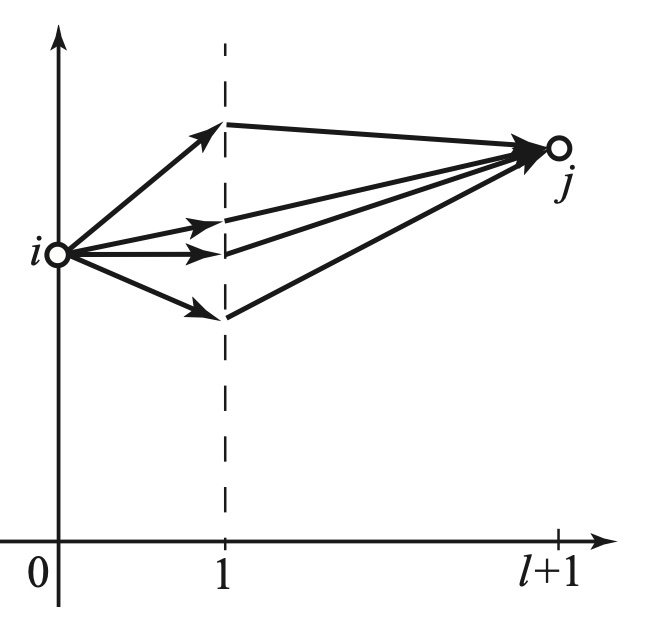
\includegraphics[width=0.5\linewidth]{Ger0r0r_pic_n_1.jpg} \\ а)}
    \end{minipage}
    \hfill
    \begin{minipage}[h]{0.49\linewidth}
    \center{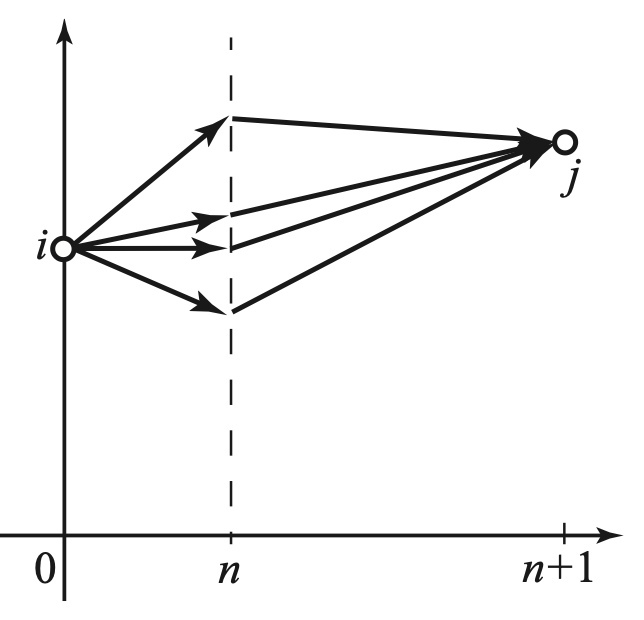
\includegraphics[width=0.5\linewidth]{Ger0r0r_pic_l_1.jpg} \\ б)}
    \end{minipage}
    \caption{а) Обратное уравнение б) Прямое уравнение}
\end{figure}

Из обратного уравнения следует
$$P^{(l)} = PP^{(l - 1)} = ... = P^l$$

где $P^{(l)} = \left| p_{ij}^{(l)}\right|$  - матрица вероятностей переходов за $l$ шагов; Р - матрица вероятностей переходов за 1 шаг. Т.е. для того, чтобы получить матрицу вероятностей переходов за $l$ шагов необходимо матрицу перехода за 1 шаг возвести в степень $l$.

\subsection{Нахождение вероятностей переходов с помощью производящих функций} 

Рассмотрим однородную цепь Маркова с дискретным временем и конечным числом состояний $X = \{1, 2, ..., N\}$. Прямое уравнение Чепмена-Колмогорова \eqref{eq-4} для нее можно переписать в виде

\begin{equation}\label{eq-5}
	p_{ij}^{(n)} = sum_{k = 1}^{N} p_{ik}^{(n - 1)}p_{kj}, i,j = \overline{1, N}, n \geq 2
\end{equation}

Данное соотношение обычно используют для вычисления $p_{ij}^{(n)}$ при небольших $n$. При больших $n$ используют следующий метод.
\par\medskip

Обозначим

\begin{equation}\label{eq-6}
    p_{ij}^{(0)} = \delta_{ij} = 
    \begin{cases}
      1, i = j
      \\
      0, i \neq j
    \end{cases}
\end{equation}

Тогда уравнение \eqref{eq-5} выполняется $при n = 1$, что можно проверить прямой подстановкой. Введем в рассмотрение производящие функции:
$$\psi_{ij}(z) = \sum_{n = 0}^{\infty} p_{ij}^{(n)}z^{n} $$

Ряд в правой части сходится по меньшей мере при $|z| < 1$, так как $0 \leq p_{ij}^{(n)} \leq 1$. Умножив обе части равнения \eqref{eq-5} на $z^{n}$ и просуммировав по $n$ от 1 до $\infty$, получим
$$\sum_{n = 1}^{\infty}p_{ij}^{(n)}z^n = \sum_{n = 1}^{\infty} \sum_{k = 1}^{N} p_{ik}^{(n - 1)}z^n p_{kj}$$

или
$$\sum_{n = 0}^{\infty}p_{ij}^{(n)}z^n -  p_{ij}^{(0)} = z \sum_{n = 0}^{\infty} \sum_{k = 1}^{N} p_{ik}^{(n)}z^n p_{kj}$$

Отсюда следует, что
$$\psi_{ij}(z) - p_{ij}^{(0)} = z \sum_{k = 1}^{N} \psi_{ik}(z) p_{kj}$$

Подставив в это равенство \eqref{eq-6}, получим

\begin{equation}\label{eq-7}
	\psi_{ij}(z) - z \sum_{k = 1}^{N} \psi_{ik}(z) p_{kj} = \delta_{ij}, i,j = \overline{1, N}
\end{equation}

Получили систему $N^2$ уравнений с $N^2$ неизвестными. Однако, так как в левую и правую часть равенства \eqref{eq-7} входит одно и то же $i$, можно отдельно решить $N$ уравнений при фиксированном $i$.
\par\medskip

Обозначим через $\Delta(z)$ определитель данной системы (один и тот же для всех $i$).

\begin{equation}\label{eq-8}
	\Delta(z) = \left|
	\begin{array}{cccc}
	1 - zp_{11} & -zp_{21} & \ldots & -zp_{N1}\\
	-zp_{12} & 1 - zp_{22} & \ldots & -zp_{N2}\\
	\vdots & \vdots & \ddots & \vdots\\
	-zp_{1N} & -zp_{2N} & \ldots & 1 - zp_{NN}
	\end{array}
	\right|
\end{equation}

При малом $|z|$ диагональные элементы близки к 1, а недиагональные - к 0, т.е. опеределитель $\Delta(z)$ близок к 1. Значит, $\Delta(z) \neq 0$ в некоторой окрестности точки $z = 0$  система уравнений \eqref{eq-7} имеет единственное решение.
\par\medskip

Так как коэффициенты этих уравнений - линейные функции, то 

\begin{equation}\label{eq-9}
	\psi_{ij}(z) = \frac{R_{ij}(z)}{S(z)}
\end{equation}

где $R_{ij}(z); S(z)$ - некоторые полиномы. Выражение \eqref{eq-9} после выделения целой части можно разложить на простейшие дроби вида $\frac{\beta_r}{(1 - \alpha_r z)^{r + 1}}$, где $\beta_r; \alpha_r$ - некоторые комплексные постоянные, $r = 0,1,2,...$.

\par\medskip

Далее будем исходить из тождества

\begin{equation}\label{eq-10}
	sum_{n = 0}^{\infty}\alpha^{n}z^{n} = \frac{1}{1 - \alpha z}
\end{equation}

Продифференцировав его $r$ раз, получим
$$\sum_{n = r}^{\infty} n(n - 1)\cdot...\cdot(n - r + 1)\alpha^{n} z^{n - r} = \frac{\alpha^{r}r!}{(1 - \alpha z)^{r + 1}} $$

или, что то же самое
$$\frac{1}{r!} \sum_{n = r}^{\infty} (n + r)(n + r - 1)\cdot...\cdot(n + 1)\alpha^{n} z^{n} = \frac{1}{(1 - \alpha z)^{r + 1}} $$

Таким образом, каждой элементарной дроби вида $\frac{\beta}{(1 - \alpha z)^{r + 1}}$, $r = 1,2,...$, соответствует составляющая $p_{ij}^{(n)}$ вида $\frac{\beta}{r!} (n + r)\cdot(n + r - 1) \cdot ... \cdot (n + 1)\alpha^{n}$; дроби вида $\frac{\beta}{1 - \alpha z}$ соответствует составляющая $p_{ij}^{(n)}$ вида $\beta \alpha^{n}$. Следовательно, $p_{ij}^{(n)}$ равно конечной сумме всех этих составляющих. 

\par\medskip
Описанным способом можно найти пределы $\lim_{n \rightarrow \infty} p_{ij}^{(n)}$, если они существуют.
